\pdfoptionpdfminorversion=7
\documentclass[sigconf, table]{acmart}


\usepackage{comment}
\usepackage{graphicx}
\usepackage{csquotes}
\usepackage{balance}
\usepackage{setspace}

\usepackage{listings}
\usepackage{subcaption}

\usepackage{standalone}

\lstset{ %
language=C++,                % choose the language of the code
basicstyle=\ttfamily\footnotesize,       % the size of the fonts that are used for the code
columns=fullflexible,
numbers=left,                   % where to put the line-numbers
numberstyle=\footnotesize,      % the size of the fonts that are used for the line-numbers
stepnumber=1,                   % the step between two line-numbers. If it is 1 each line will be numbered
numbersep=5pt,                  % how far the line-numbers are from the code
%backgroundcolor=\color{codeBG3},  % choose the background color. You must add \usepackage{color}
showspaces=false,               % show spaces adding particular underscores
showstringspaces=false,         % underline spaces within strings
showtabs=false,                 % show tabs within strings adding particular underscores
frame=single,           % adds a frame around the code
tabsize=2,          % sets default tabsize to 2 spaces
captionpos=b           % sets the caption-position to bottom
breaklines=true,        % sets automatic line breaking
breakatwhitespace=false,    % sets if automatic breaks should only happen at whitespace
keywordstyle=\color{blue},       % keyword style
  %language=Octave,                 % the language of the code
  otherkeywords={SearchVar,MV,TSS,tileExpr,Search,tFunc...},           % if you want to add more keywords to the set
  numberstyle=\tiny\color{black}, % the style that is used for the line-numbers
  rulecolor=\color{black},
escapeinside={<@}{@>}
}
\definecolor{ForestGreen}{RGB}{34,139,34}
\newcommand{\todo}[1]{{\textcolor{red}{{\tt{TODO:}}\,\,#1 }}}
\newcommand{\nc}[0]{\todo{cite}}
\newcommand{\an}[1]{{\textcolor{blue}{Author's Note: #1}}}
\newcommand{\ttt}[1]{{\texttt{#1}}}

\newcommand{\FormatDecisions}[0]{{\texttt{FormatDecisions}}~}
\graphicspath{{.}{ScoreValidity}}

\usepackage[subtle]{savetrees}

\title{Something about data layouts}


% \author{Brandon Neth}
% \affiliation{%
% 	\institution{University of Arizona}
% 	\city{Tucson}
% 	\state{AZ}
% 	\country{USA}}
% \email{brandonneth@email.arizona.edu}

% \author{Thomas R.W. Scogland}
% \affiliation{
% 	\institution{Lawrence Livermore National Laboratory}
% 	\city{Livermore}
% 	\state{CA}
% 	\country{USA}}

% \author{Bronis R. de Supinski}
% \affiliation{
% 	\institution{Lawrence Livermore National Laboratory}
% 	\city{Livermore}
% 	\state{CA}
% 	\country{USA}}

% \author{Michelle Mills Strout}
% \affiliation{%
% 	\institution{University of Arizona}
% 	\city{Tucson}
% 	\state{AZ}
% 	\country{USA}}




\begin{document}

\begin{abstract}
%In a world of ever-increasing diversity of computing platform, performance portability is of critical importance. 
%Especially in high performance computing contexts, the portability of optimizations balancing parallelism and data movement are key. 
%Such optimization portability was developed in RAJALC, an extension of RAJA incorporating the loop chain abstraction.
%This work created an inter-loop context for the purpose of schedule optimizations like loop fusion and overlapped tiling.
%While RAJALC enabled the portable specification of complex schedule changes, it left unleveraged a significant factor on performance: data layouts.
%\todo{Brandon, I am not sure we want to bring up RAJALC.  Unless the symbolic execution in RAJALC is how you
%are doing the data layout specifications and layout changes as well?  Or developing the model maybe?  The
%connection needs to be made explicit.  I take a guess in the draft intro.}



The layout of data in memory is a key consideration in high performance computing applications.
From reducing cache and page misses to relieving pressure on memory bandwidth to avoiding inter-process communication, good data layout improves performance at all levels of an application.
RAJA, a C++ performance portability library, incorporates the layout of an application's data into its definition.
This means that a developer can try out different layouts without major refactoring costs.
However, in some applications, it is beneficial to change the data layout mid-computation to facilitate better locality.
Implementing such a mid-computation layout change in RAJA can improve performance, but is laborious to implement and lacks portability.
This work remedies RAJA's shortcoming by introducing a lightweight, declarative API for changing data layouts between computations.
Also, we present an automated layout decider that selects optimal layouts based on performance estimations. 
These systems work together, meaning the decider \enquote{fills in} layout choices not made by the user.
This allows the user to specify as much or as little of the layout information as they please and still obtain the performance benefits of changing data layouts.  
Furthermore, our system is built directly into the RAJA library, meaning that no additional build steps are required.
We evaluate our system on \todo{what}, where it achieves \todo{what}.
\end{abstract}



\maketitle

\section{Introduction}

How data is stored and accesses has always been recognized to have a significant impact on performance. 
On a typical cache-based system, iterating through a two-dimensional array in column-order when data is 
stored in row-order can lead to a \todo{how much} slowdown 
\todo{cite... what if we just used our own results here? The verification of the traversal order stuff will show this}.
Although mechanisms such as compiler optimizations (loop permutation/interchange) 
and data layout policies like those in Kokkos \cite{edwards2014kokkos} and RAJA \cite{hornung2014RAJA} have the potential to align data layout with computation schedules, they become difficult to automate and laborious to manage by-hand as the number of loops and arrays grow.
\todo{Probably a good idea to refer to existing solutions to this problem as my familiarity with the literature grows}

Thus, in this paper, we present an approach for exposing data layout decisions to the programmer in the C++ performance portability library RAJA.
Our API allows the programmer to specify as many data layout decisions in a sequence of data-sharing loops (otherwise known as a loop chain~\cite{krieger2013loop}) as they choose.
Then, using a portable cost model based on microbenchmarking, our system identifies any remaining layout changes that will improve performance.  

Figure~\ref{IntroExample} shows how important good data layout is. 
The BadLayout column shows the execution time for a matrix multiplication where the three arrays are laid out opposite of their access order. 
The GoodLayout column shows the execution time for the same matrix multiplication when the arrays are laid out to match their access order.
Finally, the LayoutChange column shows the execution time of code that changes the layout from the bad layout to the good one.
As the graph shows, there is significant performance improvement ($1.51\times$ speedup) simply by changing the data layout, and the cost of performing the layout change is negligible ($1.47\times$ speedup when including conversion time). 

\begin{figure}
	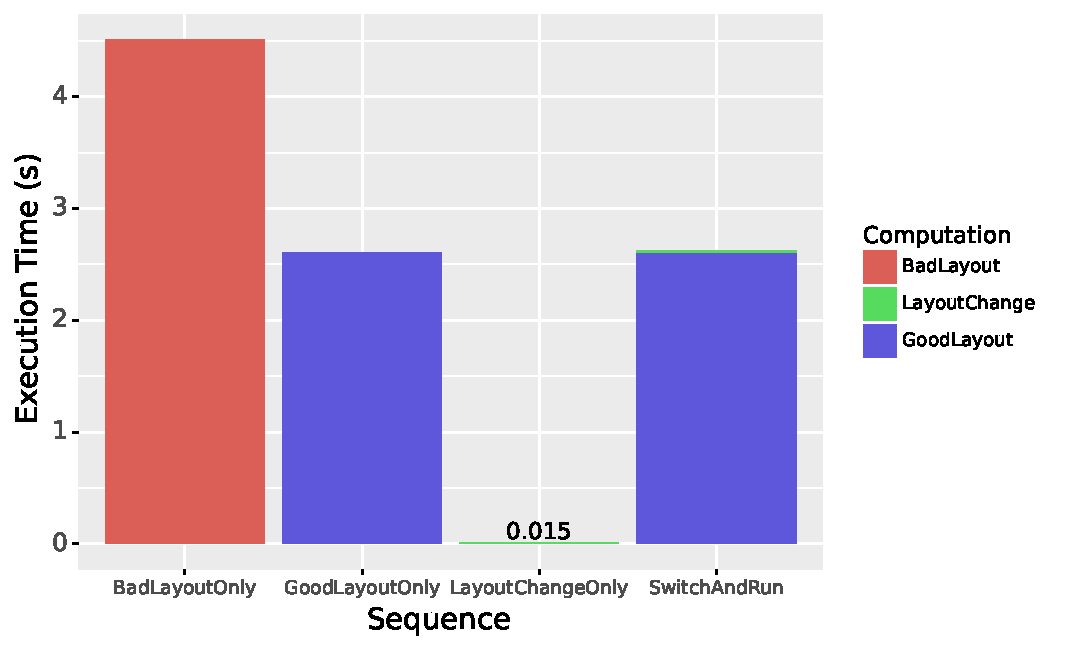
\includegraphics[width=0.7\columnwidth]{ScoreValidity/IntroExampleGraph.pdf}
	\caption{Execution time for matrix multiplication using different layouts and execution time for code changing the layouts of the same arrays.}
	\label{IntroExample}
\end{figure}

\todo{Create RUNNING EXAMPLE. I think the simpler example in figure 1 is better for the points its trying to make, but we need a running example for using our interface. I think this will separate out the claims that there is performance gains to be had from the claims that our method gives those performance gains. }
% \todo{Brandon, also we need to figure out how parallelism is related to this work, if at all.  It seems like the
% data layouts are important because of the sequential array access order.  The below introduction does NOT
% bring in parallelism yet due to my lack of understanding on this point.}

% \todo{RUNNING EXAMPLE: A paragraph showing an example sequence of loops 
% (2 would be sufficient) 
% where you can show a scatter plot of performance based on different data layout choices.  
% The Listing 1 example of 3MM would probably work.
% The main points to make
% are that which data layout is selected has a significant performance impact and that sometimes
% it is worth the cost of dynamically changing the data layout between computations.}

Although controlling data layout is quite important, the options programmers have to control
data layouts in coordination with loop schedules have limitations.

Compiler optimizations such as loop permutation have been developed to change loop
schedules so that a loop traversal order better aligns with data layout.
However, general purpose compilers (1) have difficulties analyzing for the relationship between
data layout and schedule due to things like aliasing and lack of multidimensional arrays in 
C/C++ languages, (2) do not generally expose fine-grained data layout or loop optimization
controls to users, and (3) typically do not optimize across multiple loops well.
\todo{Michelle: My understanding is that also you can't optimize two accesses at once with this method, bc changes to optimize one may un-optimize the other. Is this worth mentioning as well?}
\todo{We should have citations for these limitations probably}

Data layout policies provided in libraries like Kokkos or RAJA
and programming languages like Chapel~\cite{diaconescu2007approach} give
programmers control over the data layout of multi-dimensional arrays, but do not 
provide assistance for switching between data layouts between computations \todo{confirm for Kokkos}
nor help with selecting the most effective data layout strategy for a sequence of computations.

\todo{this paragraph seems to echo the above. I'm going to try to make it address the limitations better. Or change the flow.}
In this paper, we present an extension to the RAJA C++ library that enables a programmer
to specify the data layout for each multi-dimensional array before each 
computation\footnote{Since the control is completely exposed, an autotuner could also try out different options.}.
\todo{Show the api for specifying the best performing data layout strategy
for the RUNNING EXAMPLE.}
However, the programmer does not have to specify all data layout information, because
we also present a run-time performance model based on microbenchmarking that is
then fed into an Integer Linear Programming problem to make all of the data layout decisions
that the programmer has not made.
The performance model and ILP solver can run dynamically or ahead of time.

This paper includes the following contributions:
\begin{itemize}
\item An API in RAJA for specifying data layouts and data layout transformations.
\item A performance model to select a data layout and data layout transformation strategy for 
         a loop chain.
\item An evaluation of the performance model that shows ...\todo{how often is it right on how many architectures}
\item An optimization for reducing the amount of micro-benchmarking needed.
\item SLOC and performance results for the resulting data layouts on 3MM, ...
\end{itemize} 


%%%%%%%%%%%%%%%
\section{RAJA and RAJALC}

\begin{figure}
	\begin{lstlisting}[
		caption={Two kernels implementing matrix multiplication using different kernel policies.},
		label={MatMulTraversalOrder}]
	View2D A(A_data, layout_01);
	View2D B(B_data, layout_10);
	View2D C(C_data, layout_01);
	
	auto loop_body = [=](auto i0, auto i1, auto i2) {
		C(i0,i1) += A(i0,i2) * B(i2,i1);
	}
	
	using Policy_012 = KernelPolicy<
		statement::For<0, loop_exec,
			statement::For<1, loop_exec,
				  statement::For<2, loop_exec,
					  statement::Lambda<0>
				  >
			>
		  >
	>;
	using Policy_201 = KernelPolicy<
		statement::For<2, loop_exec,
			statement::For<0, loop_exec,
				  statement::For<1, loop_exec,
					  statement::Lambda<0>
				  >
			>
		  >
	>;
	
	auto knl1 = make_kernel<Policy_012>(bounds, loop_body);
	auto knl2 = make_kernel<Policy_201>(bounds, loop_body);
	\end{lstlisting}
\end{figure}

\todo{Introduce RAJA and RAJALC. kernel objects, symbolic evaluation, delay between specification and execution.}

We use a variety of components of RAJA and RAJALC to enable automatic data format transformations. This section reviews how a computation is described in RAJA as well as the RAJALC extensions used in this work. 

The foundational elements of RAJA are the execution constructs, \verb.forall. and \verb.kernel.. 
Implemented as templated function calls, these constructs separate the specification of the computation from the specification of its schedule. 
The user provides three pieces of information when using these constructs. 
First, they provide the execution policy as the only template argument. 
This describes the structure of a loop, including schedule choices at each nesting level. 
Second, they provide a tuple of iterators describing the loop bounds. 
Third, they provide a lambda function describing the body of the loop.
While the execution constructs immediately execute the computation they describe, RAJALC introduced wrapper objects that enable the computations to be analyzed and transformed before execution. 
The \verb.make_kernel. function seen at the end of Listing~\ref{MatMulTraversalOrder} creates one such kernel object.

RAJA also provides an array wrapper class called a View.
The View object has a number of capabilities that make it a valuable tool within RAJA codes.
First, Views use the call operator to perform memory accesses. 
By overloading this call operator for symbolic iterator types, RAJALC enabled the runtime symbolic evaluation of kernels that use Views.
RAJALC used the access information gathered from symbolic evaluation to ensure the correctness of its scheduling optimizations.
This work uses RAJALC's runtime symbolic evaluation to inform our performance model \todo{forward reference to where its discussed}.

Second, Views fully parameterize their underlying data formats with the Layout object.
Consider a programmer who wants to switch their data from row-major to column-major. 
Without Views, every access to their data \verb.A[i][j]. has to be changed to \verb.A[j][i]. \textit{and} the definition of the array needs to be changed. 
This is prohibitively expensive, especially when the programmer does not yet know the performance impact of such a decision.
With Views however, the only change the programmer needs to make is to the View's definition: The layout permutation changes from $(0,1)$ to $(1,0)$.

\section{User Specification of Data Format}

Throughout a computation, different parts of the computation access data in different orders.
For example, \todo{explain 3MM or something}.
Because different formats are optimal for different kernels, this creates an opportunity for optimization. 

However, RAJA's built-in support for changing data layouts is minimal. 
While Views can be instatiated with different layouts, changing the layout of an existing View is not as simple.
This is because changing layouts also requires reordering the underlying data to match the new layout. 
To implement such a layout change by hand requires the programmer to allocate a new temporary array, 
copy the data from the View to the temporary array in the right order, 
copy the data \textit{back} to the memory in the View, 
and then finally update the View's layout object

This work removes that barrier by expanding the declarative data optimization system begun by RAJALC.
While RAJALC tackled the problem of scheduling optimizations, we target making data format changes between computations. 
The new \verb.FormatDecisions. object is the central component of our system. 
Its instantiation takes a tuple of references to Views that are possible targets of format changes and the kernel objects that constitute the whole computation.
Two methods are used to register desired formats: \verb.set_format_before. and \verb.set_format_after..
Both take the View to be reformated, the desired format, and the computation before or after which the desired format should be used.
Once all the format choices are registered, the complete computation with the desired format conversions is generated using the \verb.finalize. method.


\begin{figure}
\begin{lstlisting}[caption={The 3MM benchmark implemented using FormatDecisions.},
	label={FormatDecisions3MM}]
auto knl1 = make_kernel<KPOL>(segs1, [=](auto i0, auto i1, auto i2) {
	E(i0, i1) += A(i0, i2) * B(i2, i1);
});
auto knl2 = make_kernel<KPOL>(segs2, [=](auto i0, auto i1, auto i2) {
	F(i0, i1) += C(i0, i2) * D(i2, i1);
});
auto knl3 = make_kernel<KPOL>(segs3, [=](auto i0, auto i1, auto i2) {
	G(i0, i1) += E(i0, i2) * F(i2, i1);
});

auto decisions = format_decisions(tie(B,D,F), knl1, knl2, knl3);

decisions.set_format_before(B, {{1,0}}, knl1);
decisions.set_format_before(D, {{1,0}}, knl2);

decisions.set_format_before(F, {{0,1}}, knl1);
decisions.set_format_after(F, {{1,0}}, knl2);

auto computation = decisions.finalize();
computation();
\end{lstlisting}
\end{figure}

\section{Performance Modeling}

In addition to the format changes registered by the user, \verb.FormatDecisions. also uses a performance model to determine if additional format changes will improve performance. 
This capability means that even without any registered format choices, \verb.FormatDecisions. often selects the same changes the user would themselves choose. 
We encode the problem as an integer linear program where the solution represents our model's pick for the optimal layouts.


We use binary decision variables representing whether or not a particular format is used at different points in the chain. 
For example, there are eight decision variables for the \verb.B. View in Listing~\ref{FormatDecisions3MM}, one for each of the two possible formats at each of the four points in the chain. 
While there are only three kernels in the chain, there is an additional point added for the \enquote{output} format that the View has after the computation is done. 
We also use decision variables to represent the required format conversions.

Four types of constraints are imposed on the decision variables.
\begin{itemize}
\item Format Uniqueness: At each time point, every View has exactly one selected format. 
\item Conversion Uniqueness: At each conversion point, every View goes through exactly one conversion.
\item Format-Conversion Matching: At each conversion point, the input format for the conversion matches the format of the immediately preceding time point. Similarly, the output format for the conversion matches the format of the immediately succeeding time point.
\item User Prescription: All user-provided format choices are met.
\end{itemize}

The objective function is constructed using the estimated cost of the format choices and conversions. 
Each decision variable is assigned a cost coefficient in the following manner.
First, we execute and time a small loop with similar access patterns to the choice, then cache the result for later decision variables.
Second, we multiply the microprofiling result by the number of iterations the choice affects.
For example, a conversion decision for \verb.B. in Listing~\ref{FormatDecisions3MM} would be multiplied by the dimensions of \verb.B..
In contrast, a format decision for \verb.B. for \verb.knl1. would be multiplied by all three loop dimensions. 
The next section discusses how we reduce the amount of microprofiling necessary to make all of the estimates.

\section{Cost Estimation}

In this section, we describe how RAJALC estimates the cost of a particular layout choice and how cost estimates are reused for multiple decision variables.
This is achieved using an access' simplified traversal order.

\subsection{Identifying an Access}
The access pattern of any View access is identified by the access argument order, the kernel policy order, and the layout order. 

The access argument order describes the order of the loop iterators in the access with respect to the parameters of the lambda. In Listing~\ref{MatMulTraversalOrder}, the accesses to \verb.A., \verb.B., and \verb.C. have access argument orders $(0,2)$, $(2,1)$, and $(0,1)$, respectively. 


The kernel policy order describes the order in which the iterators are increased. 
This is equivalent to the nesting order of a loop.
In Listing~\ref{MatMulTraversalOrder}, accesses made by \verb.knl1. have policy order $(0,1,2)$, while those mady by \verb.knl2. have policy order $(2,0,1)$.
\todo{Brandon, here I am guessing it isn't the policy name but the For loop nesting order in the KernelPolicy?}

The layout order describes the layout of data in memory. 
In Listing~\ref{MatMulTraversalOrder}, \verb.A. has layout order $(0,1)$, \verb.B. has $(1,0)$, and \verb.C. has $(0,1)$.
\todo{Brandon, how are layout\_01, etc. defined?}

For an $n$-dimensional kernel and a $d$-dimensional View, there are $n! * d! * n^d$ different combinations of policy, layout order, and access argument. 
\todo{Brandon, walk through this with the example in Listing 2.  Go ahead and list all of the possibilities.}

However, many of these accesses have similar, if not identical data access behavior. 
Thus, we can greatly reduce the number of possible accesses that may need cost estimation. 
\todo{Brandon, then for this new paragraph about reducing accesses, show some of the ones from
this list you made in the last paragraph that are going to have the same performance.}


\subsection{Traversal Order}

%Because kernel policies and access arguments are defined at compile\todo{i want to say "code writing" time here} time while layouts are mutable at runtime, we want to model all accesses as different layout choices for a single pre-selected choice of kernel policy and argument order.
The programmer decides the kernel policies and access arguments.
The piece we automate here is deciding what the data layout of the various arrays accessed by
the kernels should be at various points in the loop chain.
To do this we want to model the cost of all of the data accesses for different layout choices
given a pre-selected kernel policy and access argument order.
\todo{The reader is a bit lost at this point.  We need to give them the bigger picture earlier.}



\subsection{Simplified Traversal Order}

\todo{I would rather this come later after the main idea of how you are doing the modeling is presented.}

\subsection{Empirical Verification}

\todo{Are you verifying the reduction in microbenchmarks needed or verifying the objective function period?}
Our first reduction comes from the coupling between the access arguments and the loop iterators. We can normalize the access argument order by transforming the policy order. Using this reduction, we only need to model accesses that use the iterators in order. Listing~\ref{reduction1} shows two accesses that have the same access behavior. 

\begin{figure}
	\begin{lstlisting}[caption={Equivalent loops for first reduction process.}, label={reduction1}]
kernel<POLICY_01>(... [](auto i0, auto i1) {
		a(i1,i0)
});

kernel<POLICY_10>(... [](auto i0, auto i1) {
		a(i0,i1)
});
	\end{lstlisting}
\end{figure}

The second reduction comes from the similarity between 
\begin{figure}
	\begin{lstlisting}[caption={Equivalent loops for second reduction process.}, label={reduction2}]
kernel<POLICY_012>(... [](auto i0, auto i1, auto i2) {
		a(i0,i2)
});

kernel<POLICY_01>(... [](auto i0, auto i1) {
		a(i0,i1)
});
	\end{lstlisting}
\end{figure}


\subsection{Deriving the Traversal Order}

\todo{Brandon, who is deriving the traversal order?  Symbolic execution?}
Given an $n$-dimensional kernel that accesses a $d$-dimensional view, there are $n! * d!$ different possible combinations of kernel policy and data layout. 
Estimating the cost of all of these choices separately for each access in a computation is prohibitively expensive, especially using any sort of dynamic benchmarking. 
However, the traversal order of an access compresses the kernel policy and data layout into a single reusable feature that accurately predicts relative performance.




Listing~\ref{MatMulTraversalOrder} shows two implementations of a matrix multiplication using different kernel policies and involving views using different data layouts.
Deriving the traversal order for an access requires the extraction of three values: the policy order, the layout order, and the argument order. 
For the access to \verb.C. in \verb.knl1., the policy order is $(0,1,2)$, the layout order is $(0,1)$, and the argument order is $(0,1)$. 
In contrast, for the access to \verb.B. in \verb.knl2., the policy order is $(2,0,1)$, the layout order is $(1,0)$, and the argument order is $(2,1)$. 

With these values in hand, we can derive the traversal order, using the access to \verb.B. in \verb.knl2. as a running example. 
We start with the argument order $(2,1)$.
The first step is to normalize the policy order.
This step gives us the answer to the question: \enquote{What access has the same traversal order when the policy order is monotonically increasing (the normal policy order)?}
This is calculated using the following: \verb,[policy_order.indexof(arg) for arg in arg_order],. 
The index of $2$ in the policy is $0$, and the index of $1$ in the policy is $2$, so our intermediate value is $(0,2)$. 

The second step is to permute this intermediate value based on the data layout. 
We apply the layout permutation $(1,0)$ to our intermediate value $(0,2)$ to get our traversal order $(2,0)$. 
This traversal order tells us that in the access to \verb.B. in \verb.knl2., the dimension of \verb.B. with the largest stride is traversed by the iterator at nesting depth 2 (the innermost iterator) and the dimension of \verb.B. with the smallest stride is traversed by the iterator at nesting depth 0 (the outermost iterator). 

\subsection{Traversal Order as a Performance Metric}

\todo{Brandon, this motivation needs to come a lot earlier in the paper.}
Our claim is that the traversal order of an access is an accurate predictive metric for the relative performance of a layout choice. 
We support this claim empirically using performance data from three microbenchmarks.
For each microbenchmark, we record the 5-run average execution time of every combination of kernel policy and data layout. 
These execution times are then grouped by traversal order.
If our claim is valid, then the execution times for each traversal order will cluster and the groups of execution times will not overlap.

Microbenchmark 1 is an access to a 3-dimensional view in a 3-dimensional loop. 
Microbenchmark 2 is an access to a 2-dimensional view in a 3-dimensional loop, as in a matrix multiplication.
Microbenchmark 3 is an access to a 3-dimensional view in a 4-dimensional loop.


\begin{figure}
% 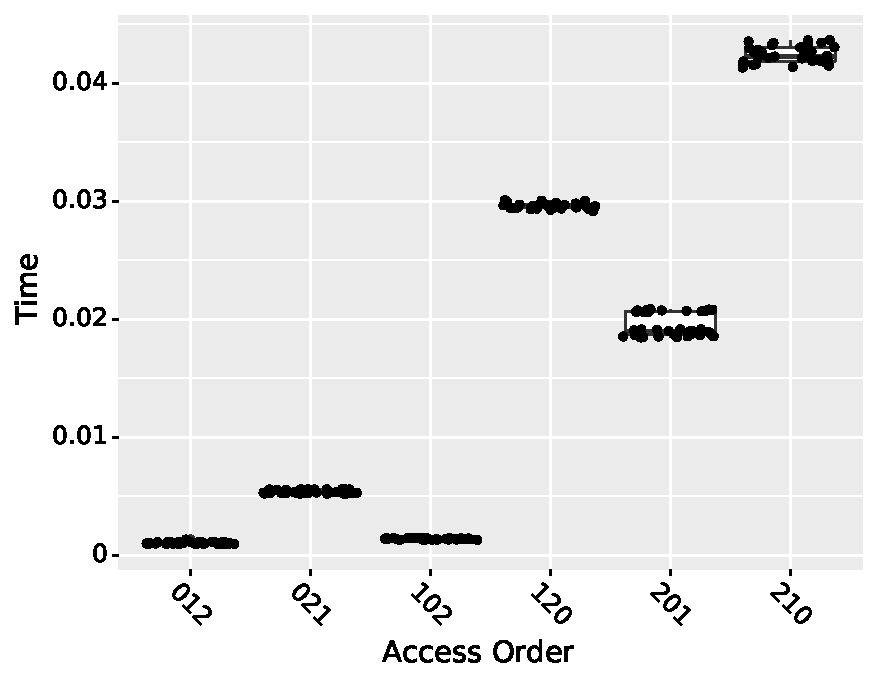
\includegraphics{benchmark1_boxplot.pdf}
\caption{Execution times for 3-dimensional loop accessing 3-dimensional view, grouped by traversal order.}
\label{TraversalBenchmark1}
\end{figure}

\begin{figure}
	% 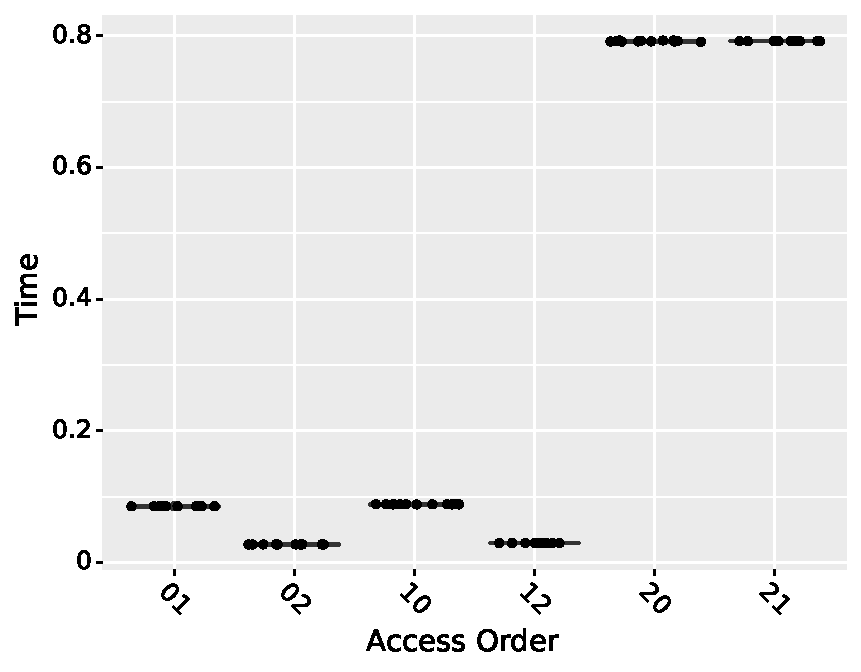
\includegraphics{benchmark2_boxplot.pdf}
	\caption{Execution times for 3-dimensional loop accessing 2-dimensional view, grouped by traversal order.}
	\label{TraversalBenchmark2}
\end{figure}

\begin{figure}
	% 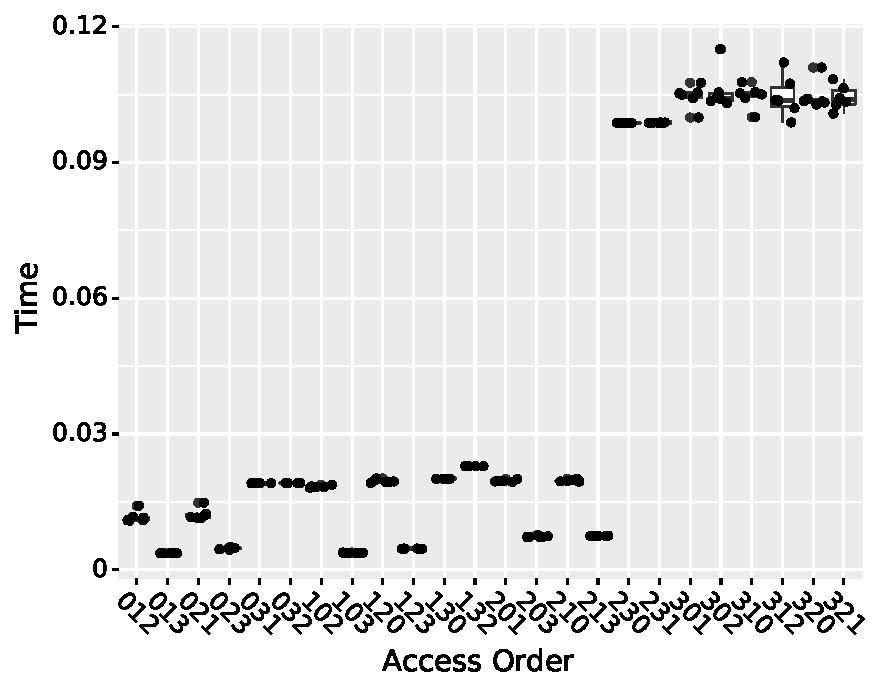
\includegraphics{benchmark3_boxplot.pdf}
	\caption{Execution times for 4-dimensional loop accessing 3-dimensional view, grouped by traversal order.}
	\label{TraversalBenchmark3}
\end{figure}

Figure~\ref{TraversalBenchmark1} shows the execution times for the different traversal orders for microbenchmark 1. 
With the exception of traversal order $(2,1,0)$, the traversal orders show good clustering.
\todo{explanation for why the $(2,1,0)$ ones don't cluster as much}
Also, the six possible traversal orders show good differentiation, with the exception of $(0,1,2)$ and $(1,0,2)$. 
This is likely because the bulk of the performance improvement comes from the innermost loop in a nest traversing the stride 1 dimension of the data.


\todo{Brandon, I am not seeing these figures right now.  Have they not been included into the repository yet?}
Figure~\ref{TraversalBenchmark2} shows the execution times for the different traversal orders for microbenchmark 2. 
While the traversal orders for this microbenchmark are all highly clustered, they are less differentiated from one another. 
For example, we see that the orders $(0,2)$ and $(1,2)$ have similar performance, as do $(2,0)$ and $(2,1)$. 
The similarity in performance is again attributable to the influence of the position of the innermost loop iterator. 



Figure~\ref{TraversalBenchmark3} shows the execution times for the different traversal orders for microbenchmark 3. 
A similar pattern as the previous microbenchmarks emerges here: grouping based on the position of the innermost iterator. 

The major benefit of using traversal order as a performance metric is its reusability. 
Because it condenses the policy, the layout, and the arguments used in the access into a single metric, the same benchmarking results can be used to estimate the cost of all three accesses within a matrix multiplication. 
Similarly, the benchmarking results for traversal orders gathered for one computation can be reused when modeling another computation.

\section{A Performance Model for Data Format}
\todo{Brandon, this is one of the key contributions of this paper and it is buried right now.}

\todo{explain how we use the traversal order information to build up a model and choose layouts and generate the computation}

\section{Evaluation}

\todo{Where we evaluated}

We evaluate our contribution on three codes: the polybench suite\nc, Kripke\nc, and miniWeather\nc.


\subsection{Evaluation Metrics}
When evaluating our systems, we consider a number of metrics. 
First,  we measure the source lines of code (SLOC) added, removed, and changed to implement layout changes by hand and using our \FormatDecisions interface.
Second, we measure the relative performance improvement between implementing layout changes by hand and using \FormatDecisions. 
This result shows the cost of modeling overhead.
Third, we measure the accuracy of our model on its own by determining the rank of its choices among all possible choices.
\todo{The explanation of the model accuracy measurement needs work.} 

\subsection{Case Study 1: Polybench}

Our first evaluation targeted the kernels within the Polybench suite. 
Polybench contains 30 numerical computations in total. 
Of those 30, 13 have good traversal orders for all multi-dimensional accesses, one uses only 1D data, and one uses external functions that inhibit RAJALC's symbolic evaluation.
This leaves 15 benchmarks to evaluate.

We evaluated the performance of three variants of the benchmarks.
The first variant, \verb.RAJA_OpenMP., is the original RAJA implementation of the kernel.
The second variant, \verb.Hand_Layout., implements the layout changes by hand.
The third variant, \verb.Auto_Layout., implements the layout changes using our contribution.



\todo{This table is temporary.}
\begin{figure*}
\begin{tabular}{ll}
Benchmark   & Inclusion \\
2mm         & Yes          \\
3mm         & Yes          \\
adi         & Yes          \\
atax        & No, accesses to A are in-order.          \\
bicg        & No, accesses to A are in-order.          \\
cholesky    & No, accesses to A are in-order.          \\
correlation & Yes          \\
covariance  & Yes          \\
deriche     & No, accesses to all multi-dimensional data are in-order.          \\
doitgen     & Yes          \\
durbin      & No, all 1D data.          \\
fdtd-2d     & No, accesses to all multi-dimensional data are in-order.           \\
floyd-warshall & No, accesses are in order \\
gemm        &  No, accesses are all in order         \\
gemver      & Yes          \\
gesummv     & No, accesses are all in order          \\
gramschmidt & Yes          \\
heat-3d     & No, accesses are all in order            \\
jacobi-1D   & No, accesses are all in order           \\
jacobi-2D   & No, accesses are all in order           \\
lu          & Yes         \\
ludcmp      & Yes          \\
mvt         & Yes          \\
nussinov    & No, too much control flow and function calls          \\
seidel      & No, accesses are all in order           \\
symm        & Yes          \\
syr2k       & Yes          \\
syrk        & Yes          \\
trisolv     & No, accesses are all in order           \\
trmm        & Yes         
\end{tabular}
\caption{Polybench benchmarks}
\end{figure*}


\subsection{Case Study 2: miniWeather}

\subsection{Case Study 3: Kripke}

\section{Related Work}

Kennedy and Kremer~\cite{kennedy1995automatic} developed an approach for automatically selecting data layouts for distributed arrays within High Performance Fortran (HPF). 
The high level optimization framework is similar to ours: breaking the program into segments, constructing a search space of layouts for each segment, estimating the cost of each layout choice, and selecting one candidate for each segment so that overall cost is minimized. 
Because they target distributed arrays, their approach considers the alignment of arrays with each other, while our approach considers the direct striding costs of each array separately. 

Chen, Ozturk, and Kandemir~\cite{Chen2004ilp} develop a model of locality using a 0-1 ILP formulation. 
Their decision variables indicate mappings between data elements and memory as well as scheduling choices surrounding when data elements are accessed. 
In their formulation, each data element is considered independently, meaning each array element has its own decision variable. 
Furthermore they assume complete flexibility of data ordering in memory, meaning there are no restrictions on array data being stored together.

Unat et. al.~\cite{unat2017trends} review trends in HPC related to data locality. They provide a variety of definitions which we utilize in our work. However, their definition of traversal order is not quite in line with RAJA's layout types, as layout changes affect the traversal order without changing the indices used. 
\section{Conclusion}


\bibliographystyle{abbrv}
\bibliography{DataRAJALC}
\end{document}
